\documentclass[main.tex]{subfiles} % Subfile-Class


% ============================================================================== %
%                            Subfile document                                    %
% ============================================================================== %

\begin{document}

% Template

\subsubsection{Antriebe und Dimensionierung}

Dieser Abschnitt behandelt die Auswahl eines geeigneten Antriebs mit Steuerung
für den Roboter. Die Evaluation der Antriebe, siehe
Anhang~\ref{appendix:Antriebe}, hat ergeben, dass ein Schrittmotor der Firma
DFRobot, siehe Abbildung~\ref{Schrittmotor_FIT0278}, eingesetzt wird. Dieser
ist in der Lage, den Roboter mit 1.7A auf bis zu $2\frac{m}{s}$ zu
beschleunigen.

\begin{figure}[H]
    \centering
    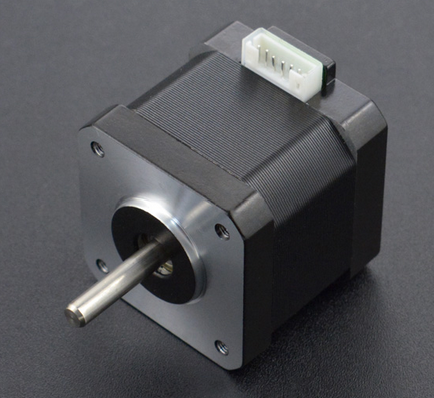
\includegraphics[width = 0.25 \linewidth]{fig_Antriebe_und_Dimensionierung/DFRobot_Stepper_FIT0278.png}
    \caption{Schrittmotor}~\label{Schrittmotor_FIT0278}
\end{figure}

\begin{figure}[H]
    \centering
    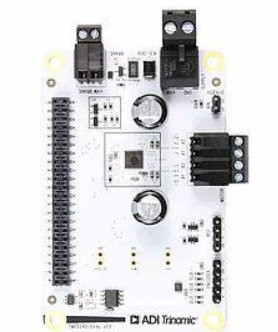
\includegraphics[width = 0.25 \linewidth]{fig_Antriebe_und_Dimensionierung/TMC_5240_EVAL.png}
    \caption{Evaluationboard TMC5240}~\label{Schrittmotorentreiber_EVAL}
\end{figure}

Die Ansteuerung dieser Motoren erfolgt über einen vollintegrierten
Schrittmotortreiber der Firma ADI-Trinamic. Um den Entwicklungsaufwand gering
zu halten, wird auf 2 Evaluation-Boards des Treiber-IC's \textit{TMC-5240}
zurückgegriffen, wie in Abbildung~\ref{Schrittmotorentreiber_EVAL} gezeigt.
Eines der Teammitglieder hat bereits Erfahrung mit diesem speziellen Treiber
und kann auf entsprechende Treiber-Evaluation-Boards aus seinem beruflichen
Umfeld zurückgreifen.

Abbildung~\ref{Ansteuerungstopologie_Schrittmotorentreiber} zeigt schematisch,
wie diese Treiber angesteuert werden.

\begin{figure}[H]
    \centering
    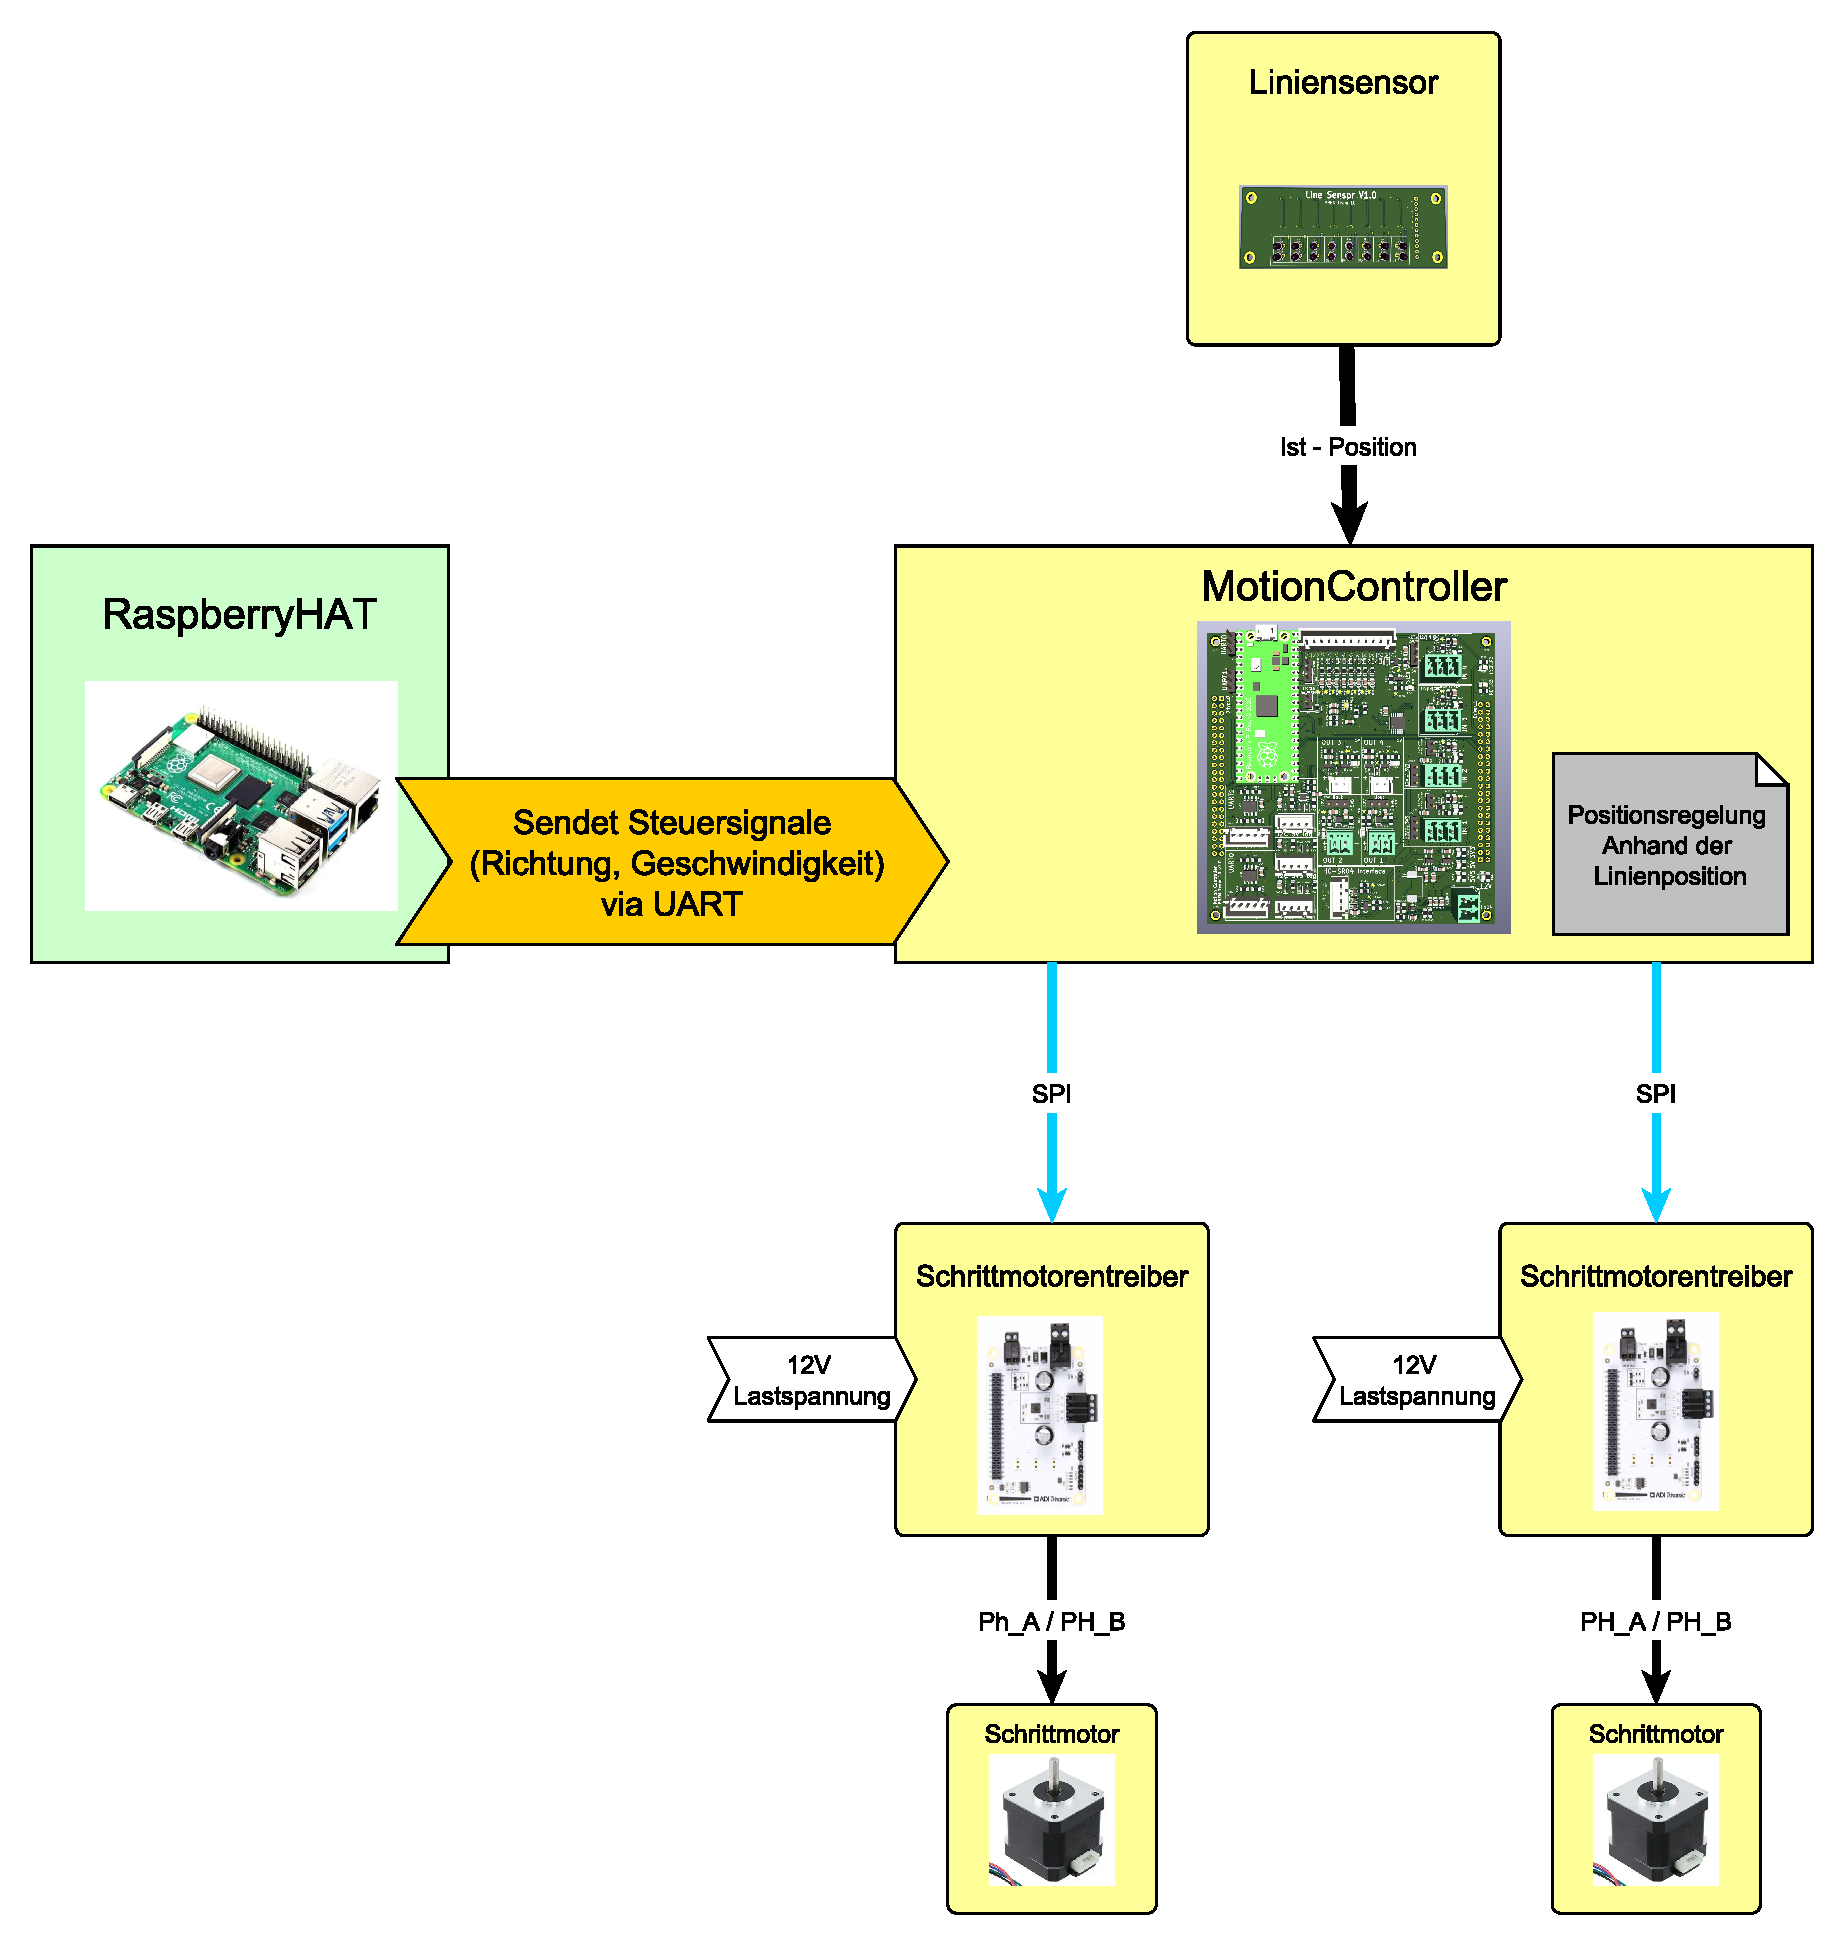
\includegraphics[width = 1\linewidth]{fig_Antriebe_und_Dimensionierung/Konzept_Motoransteuerung.pdf}
    \caption{Ansteuerungstopologie Schrittmotoren}~\label{Ansteuerungstopologie_Schrittmotorentreiber}
\end{figure}

Die Antriebsregelung ist auf einer separaten Leiterplatte realisiert. Als
Eingangssignal für diese Regelung arbeitet einzig der Liniensensor. Die
Ansteuerung der beiden Schrittmotortreiber erfolgt über den SPI-Bus des
Mikrocontrollers.

An den Rädern sind ebenfalls Encoder vorgesehen, damit der Navigationsrechner
den zurückgelegten Weg nachvollziehen kann. Aus Gründen der Echtzeitfähigkeit
bei der Auswertung der Encoder werden diese auf der Antriebssteuerung und nicht
auf dem Navigationsrechner ausgewertet. Die Encoder stellen im aktuellen
Projektstand eine Fallback-Lösung dar. Im Folgemodul wird noch evaluiert, ob
die gefahrenen Schritte, die aus dem Motortreiber ausgelesen werden können,
ausreichen, um die gefahrene Strecke nachvollziehen zu können.

Signale, in welche Richtung das Fahrzeug bewegt werden soll, sowie Start- und
Stoppsignale erhält der Mikrocontroller vom Navigationsrechner über eine
UART-Schnittstelle. Ebenfalls über UART kann der Greifcontroller Signale an den
Antriebscontroller senden, die die Antriebe stoppen - das Fahrzeug drehen oder
weiterfahren lassen.

Abbildung~\ref{fig:Blockschaltbild_Motioncontroller}zeigt schematisch, welche
Funktionsgruppen auf der entsprechenden Platine enthalten sind.

\begin{figure}[H]
    \centering
    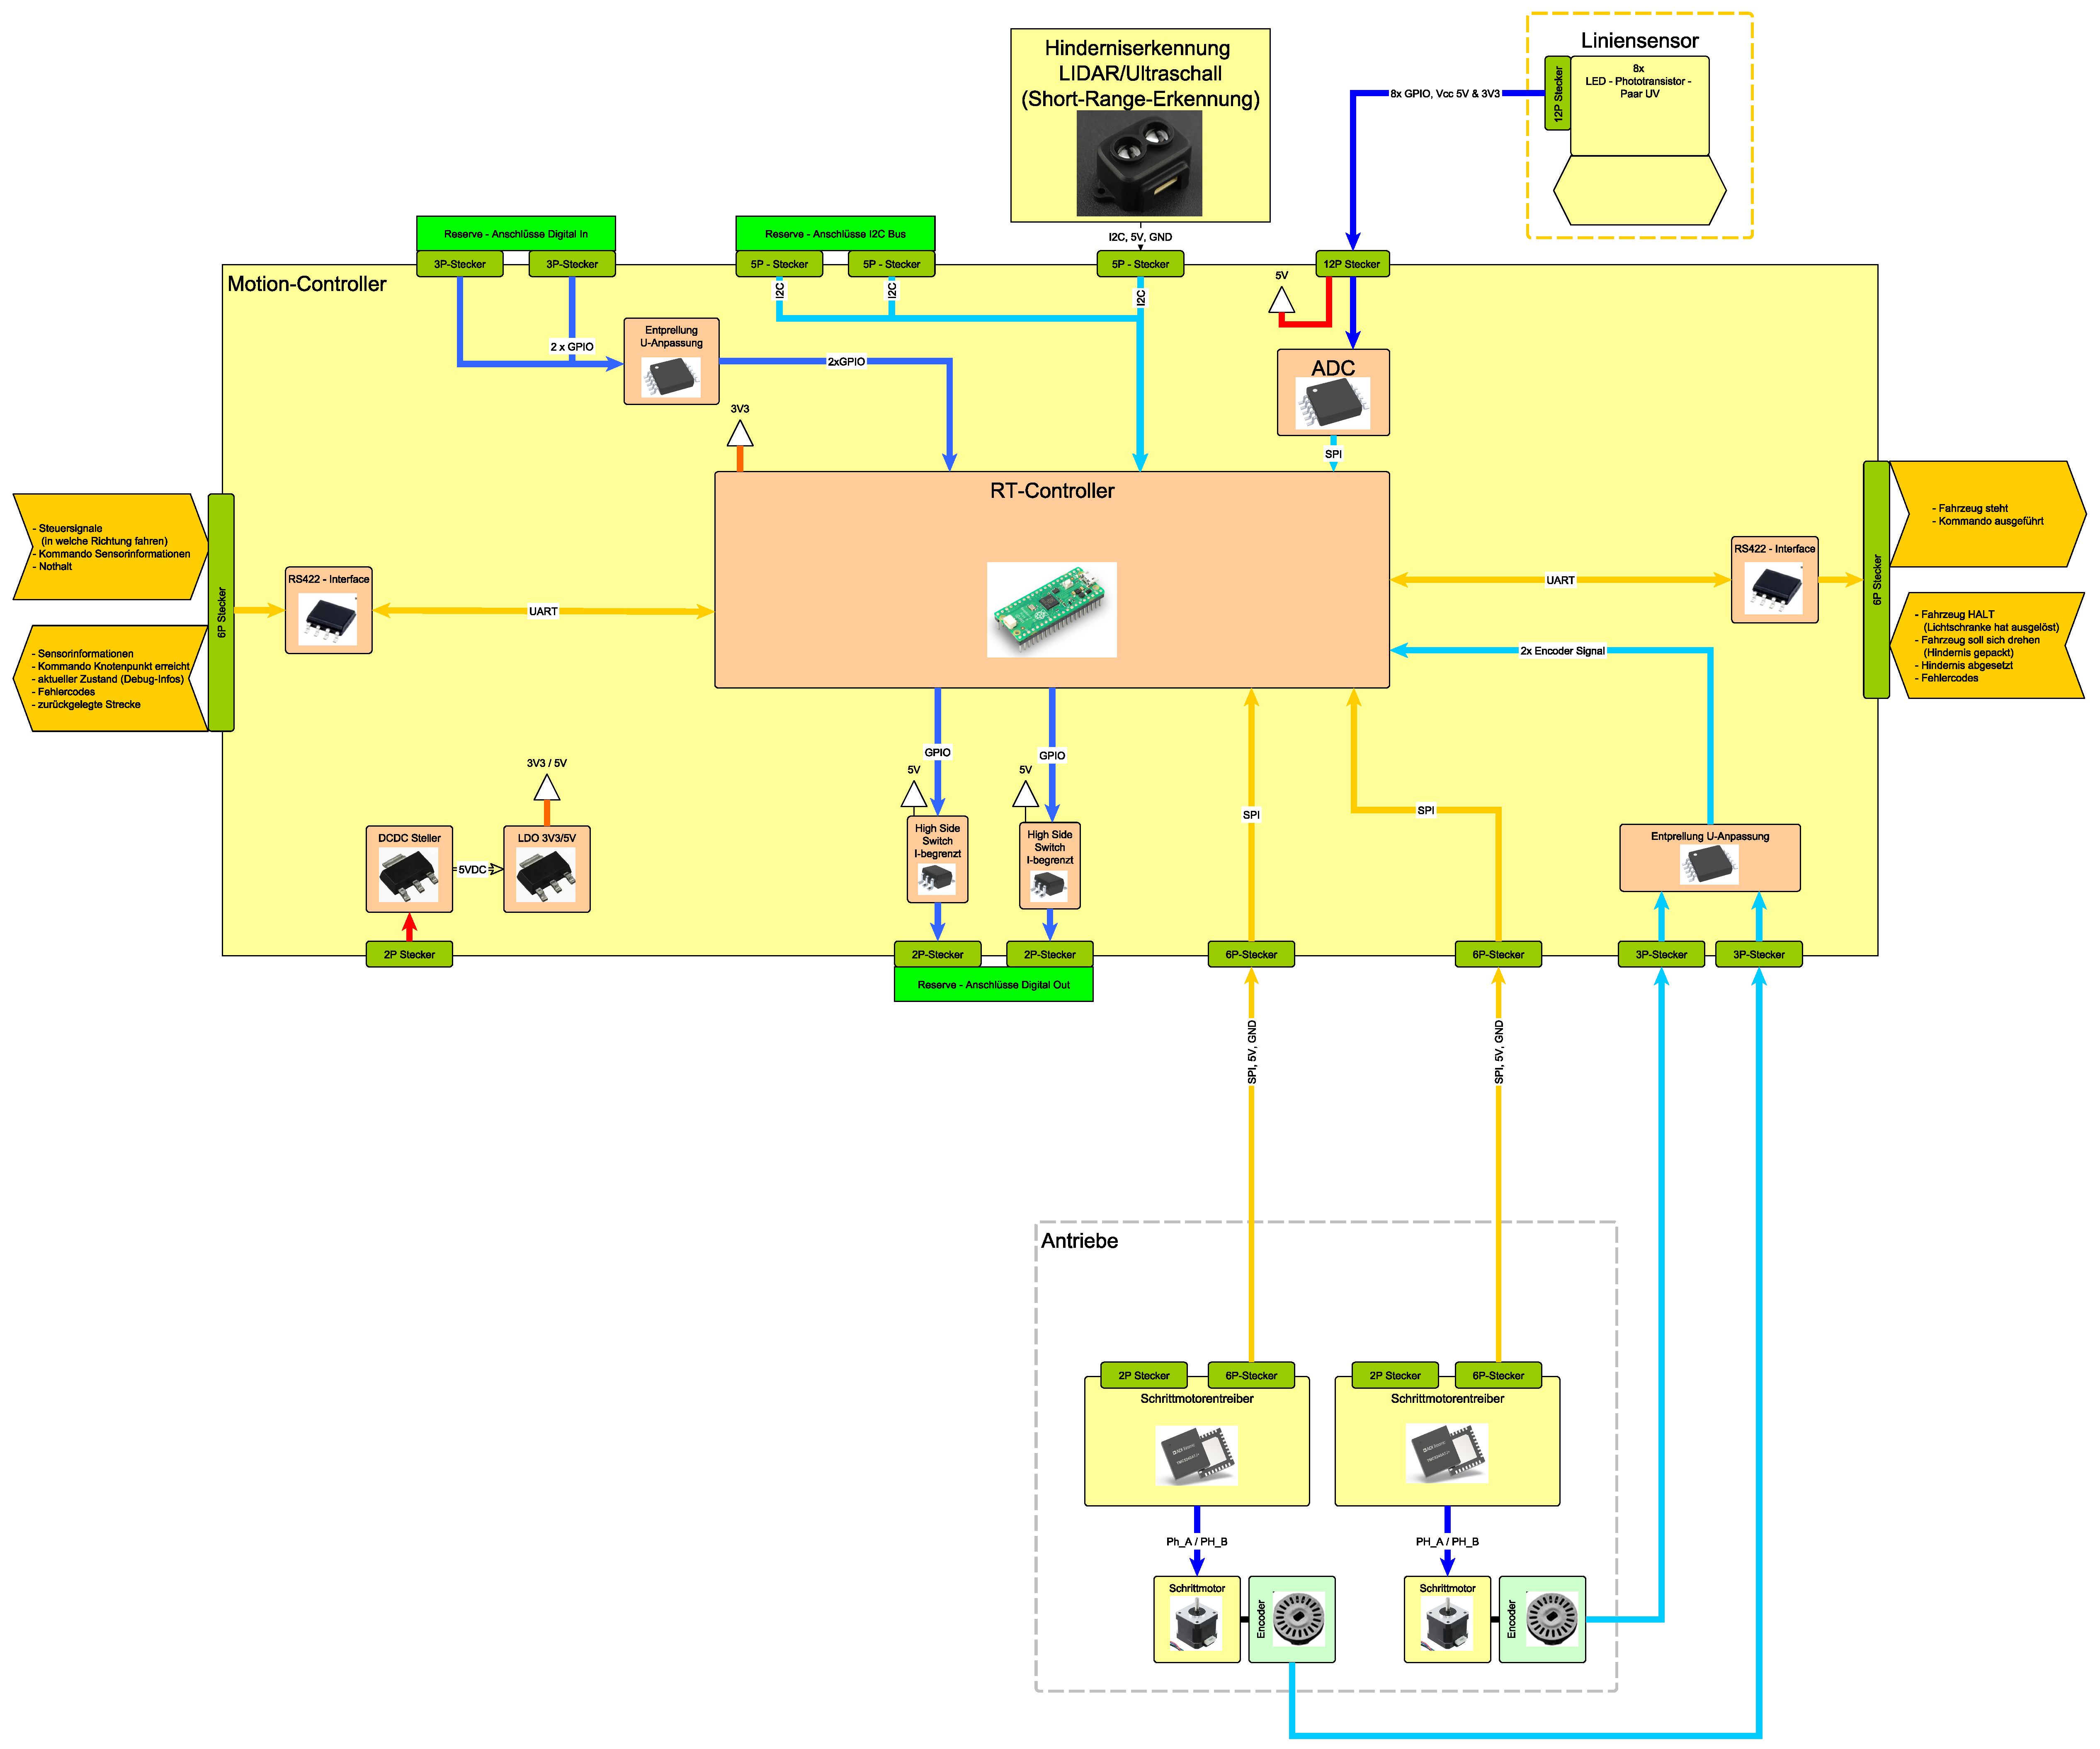
\includegraphics[width = 1\linewidth]{fig_Antriebe_und_Dimensionierung/MotionController_Blockschaltbild.pdf}
    \caption{Blockschaltbild Motion Controller}~\label{fig:Blockschaltbild_Motioncontroller}
\end{figure}

Der Motion Controller verfügt über digitale Ein- und Ausgänge mit umschaltbaren
Spannungspegeln als Reserve, falls im Verlauf des Folgemoduls PREN2 Sensoren
angepasst oder zusätzliche Aktoren hinzugefügt werden müssen.

Abbildung~\ref{fig:MotionBoard_PCB} zeigt das Motion Controller PCB in einer
3D-Ansicht. Es besitzt 3 $I^2C$-Anschlüsse, eine spezielle HC-SR04
Ultraschallsensor-Schnittstelle sowie die bereits erwähnten digitalen
Ein-/Ausgänge. Zusätzlich ist eine Schnittstelle für den Liniensensor
vorgesehen und ein Gyroskop zur Winkelerfassung integriert. Es wird wie eine
Brücke auf die beiden Evaluation Boards von Trinamic gesteckt, wofür sich die
breiten Steckerleisten an den äusseren Rändern befinden.

\begin{figure}[H]
    \centering
    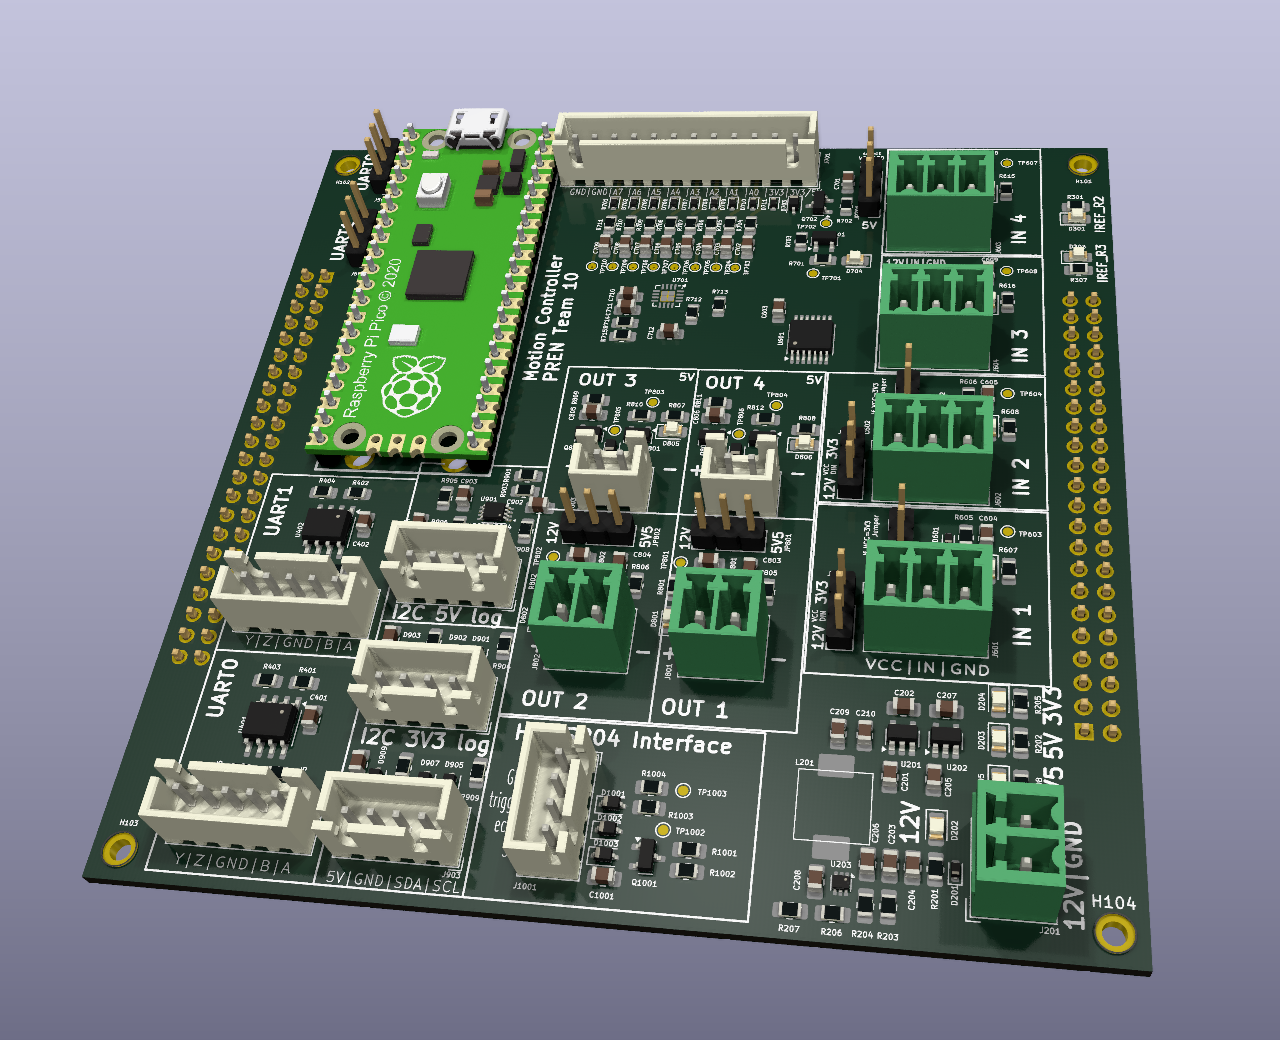
\includegraphics[width = 0.75\linewidth]{fig_Antriebe_und_Dimensionierung/MotionControllerPCB.jpg}
    \caption{3D-Ansicht Motion Controller}~\label{fig:MotionBoard_PCB}
\end{figure}

\end{document}

Nach dem derzeitigen Stand des Konzepts für PREN1 wäre dieser Controller in der
Lage, auch die Aufgabe des Greifers zu übernehmen. Es ist jedoch nicht ganz
klar, inwieweit der Greifer in seinem jetzigen Zustand implementiert werden
kann und ob noch weitere Ein-/Ausgänge benötigt werden. Daher ist für das
Folgemodul eine eigene Leiterplatte für die Greiferaufgabe vorgesehen.

\subsubsection*{Software}

Geplant ist, im Nachfolgemodul die Firmware des MotionControllers, geschrieben
in C++, auf der Basis des FreeRTOS Kernels aufzubauen.

\begin{figure}[H]
    \centering
    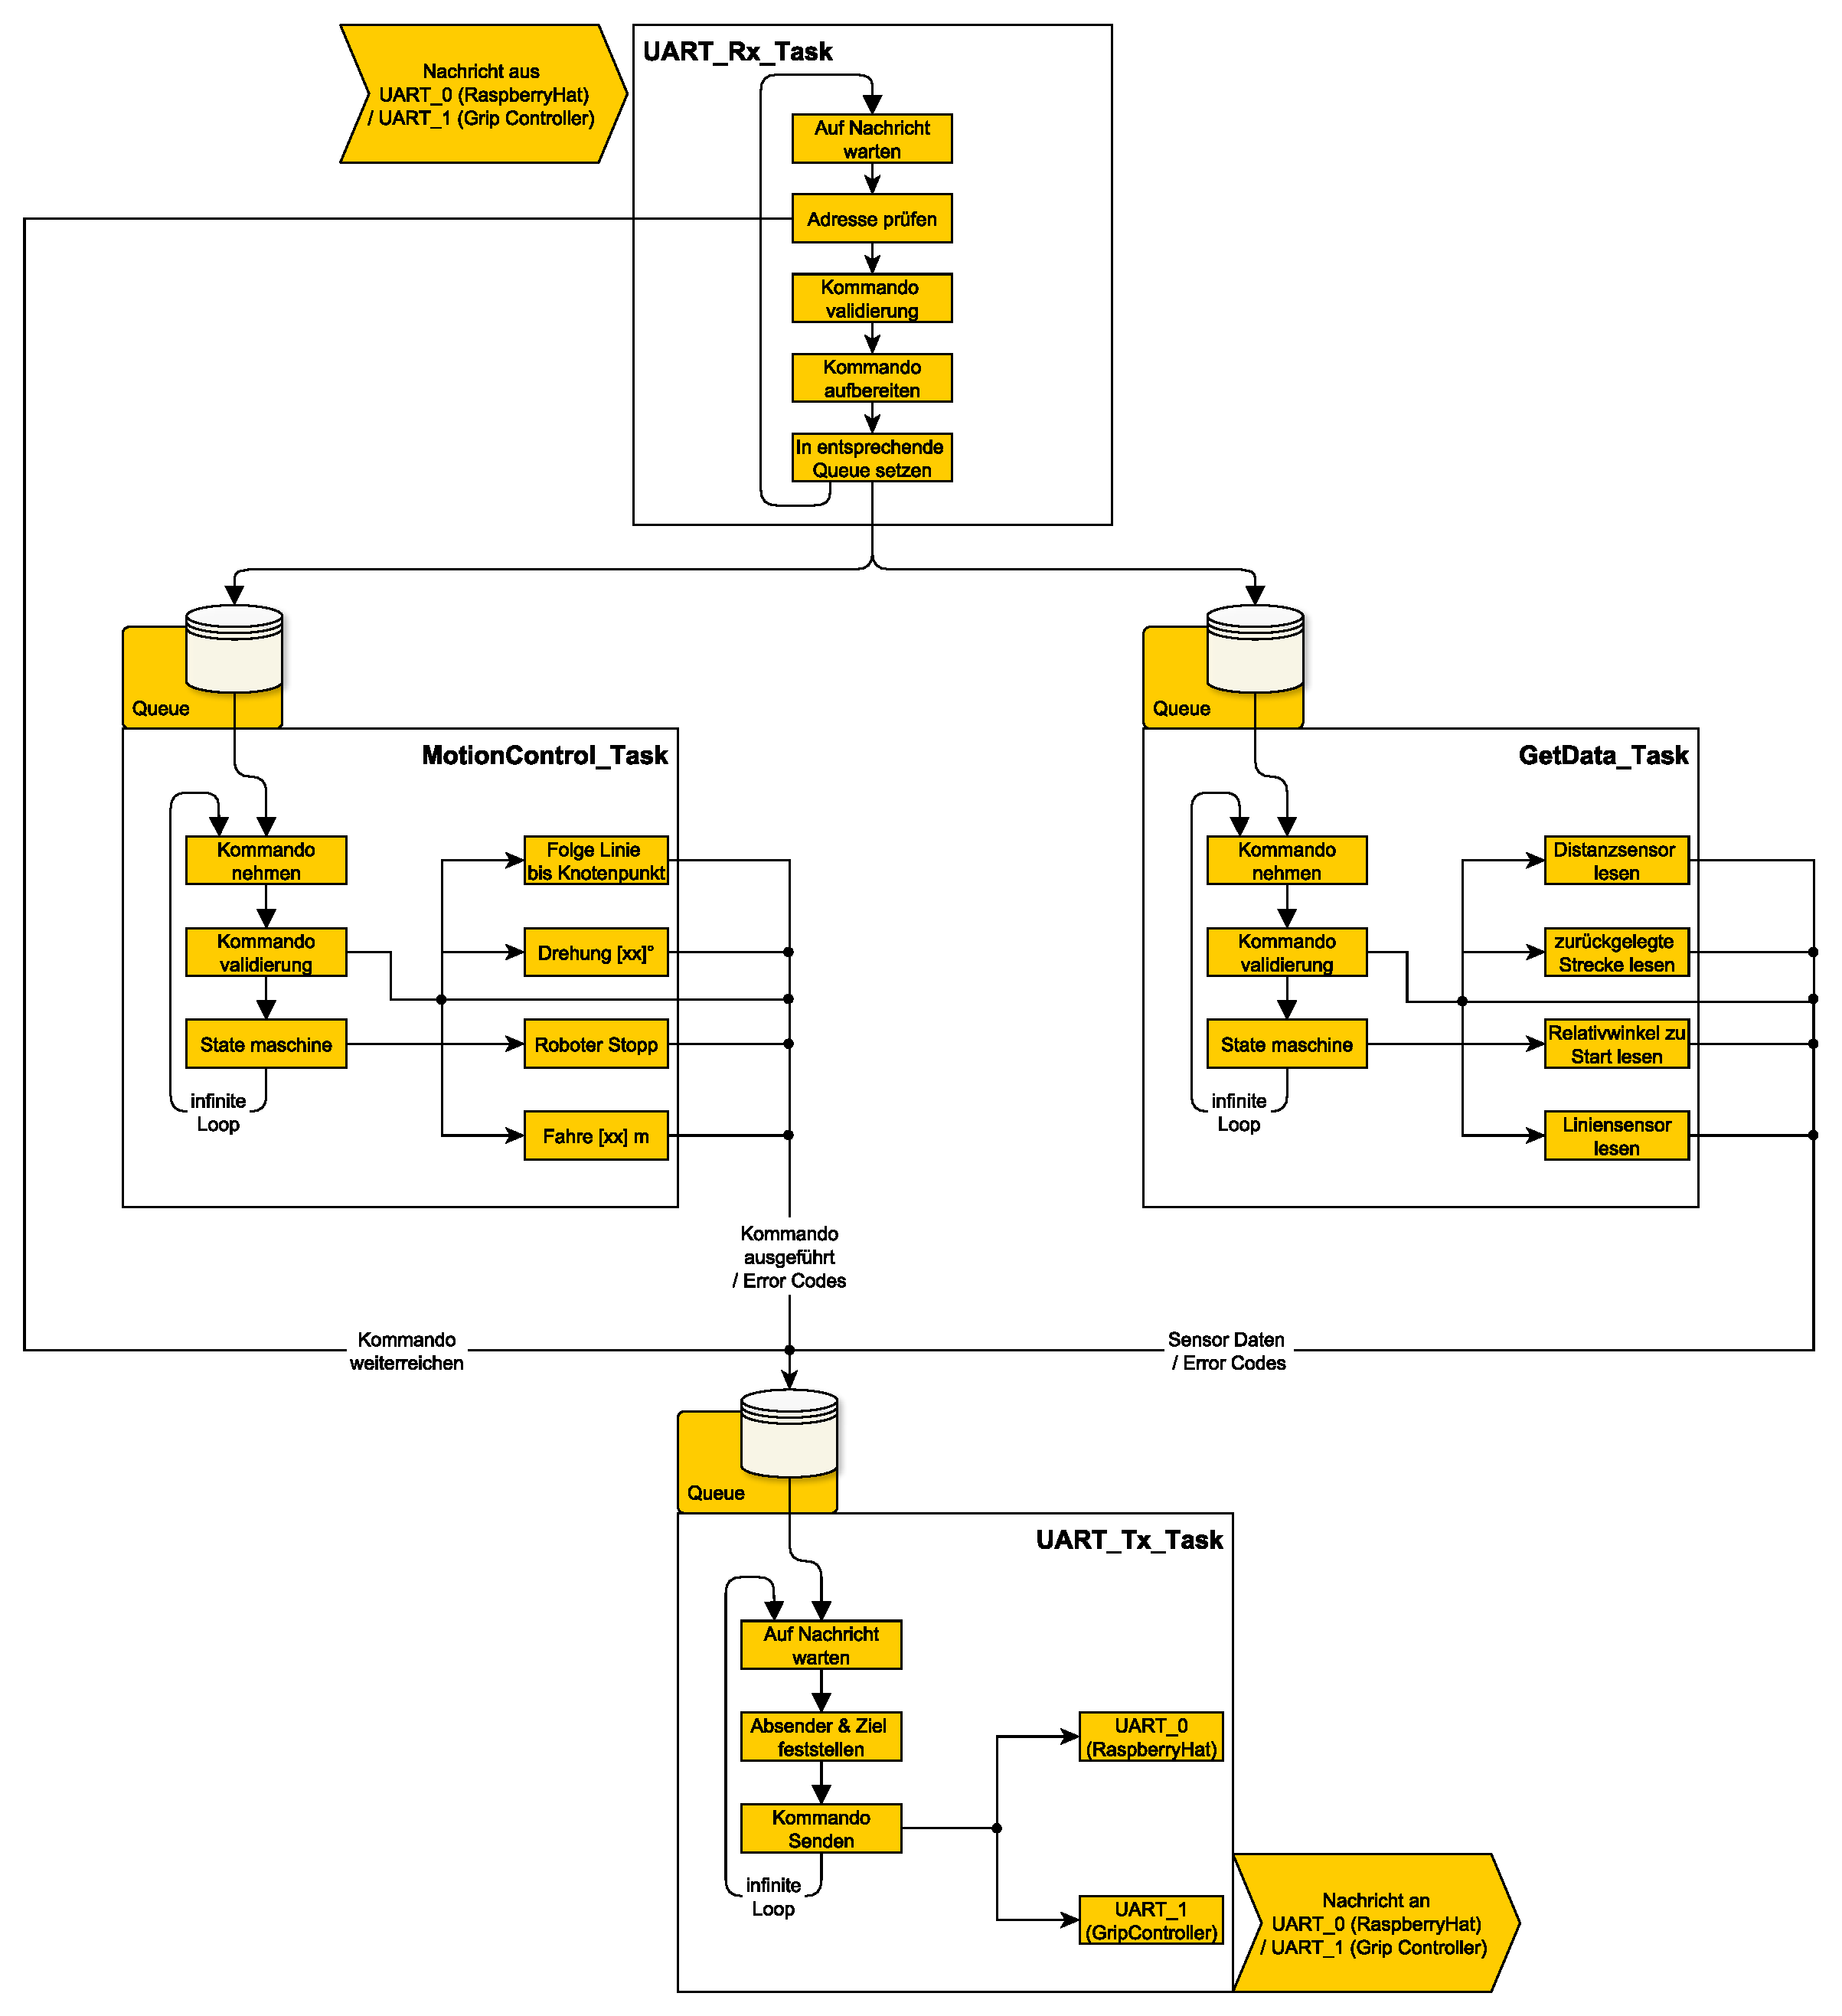
\includegraphics[width = 0.75\linewidth]{fig_Antriebe_und_Dimensionierung/Konzept_Steuerablauf.pdf}
    \caption{Steuerablauf Motion Controller}~\label{fig:MotionController_Firmware}
\end{figure}

Abbildung~\ref{fig:MotionController_Firmware} zeigt schematisch, wie die
Firmware des Motion Controllers zu implementieren ist. Es soll einen
\textit{UART_rx} und einen \textit{UART_tx} Task geben, die nur auf eingehende
und ausgehende Signale warten. Dadurch wird verhindert, dass mehrere Tasks
gleichzeitig auf dieselbe UART-Schnittstelle zugreifen. Ist der Befehl für die
Steuerung bestimmt und validiert, wird er in eine Queue eingereiht. Die
zugehörige Task arbeitet dann in Form einer Zustandsmaschine die eingehenden
Kommandos in ihrer Queue ab. Durch diesen Aufbau ist die Firmware sehr modular
aufgebaut, was spätere Anpassungen oder Erweiterungen wesentlich vereinfacht.

\begin{figure}[H]
    \centering
    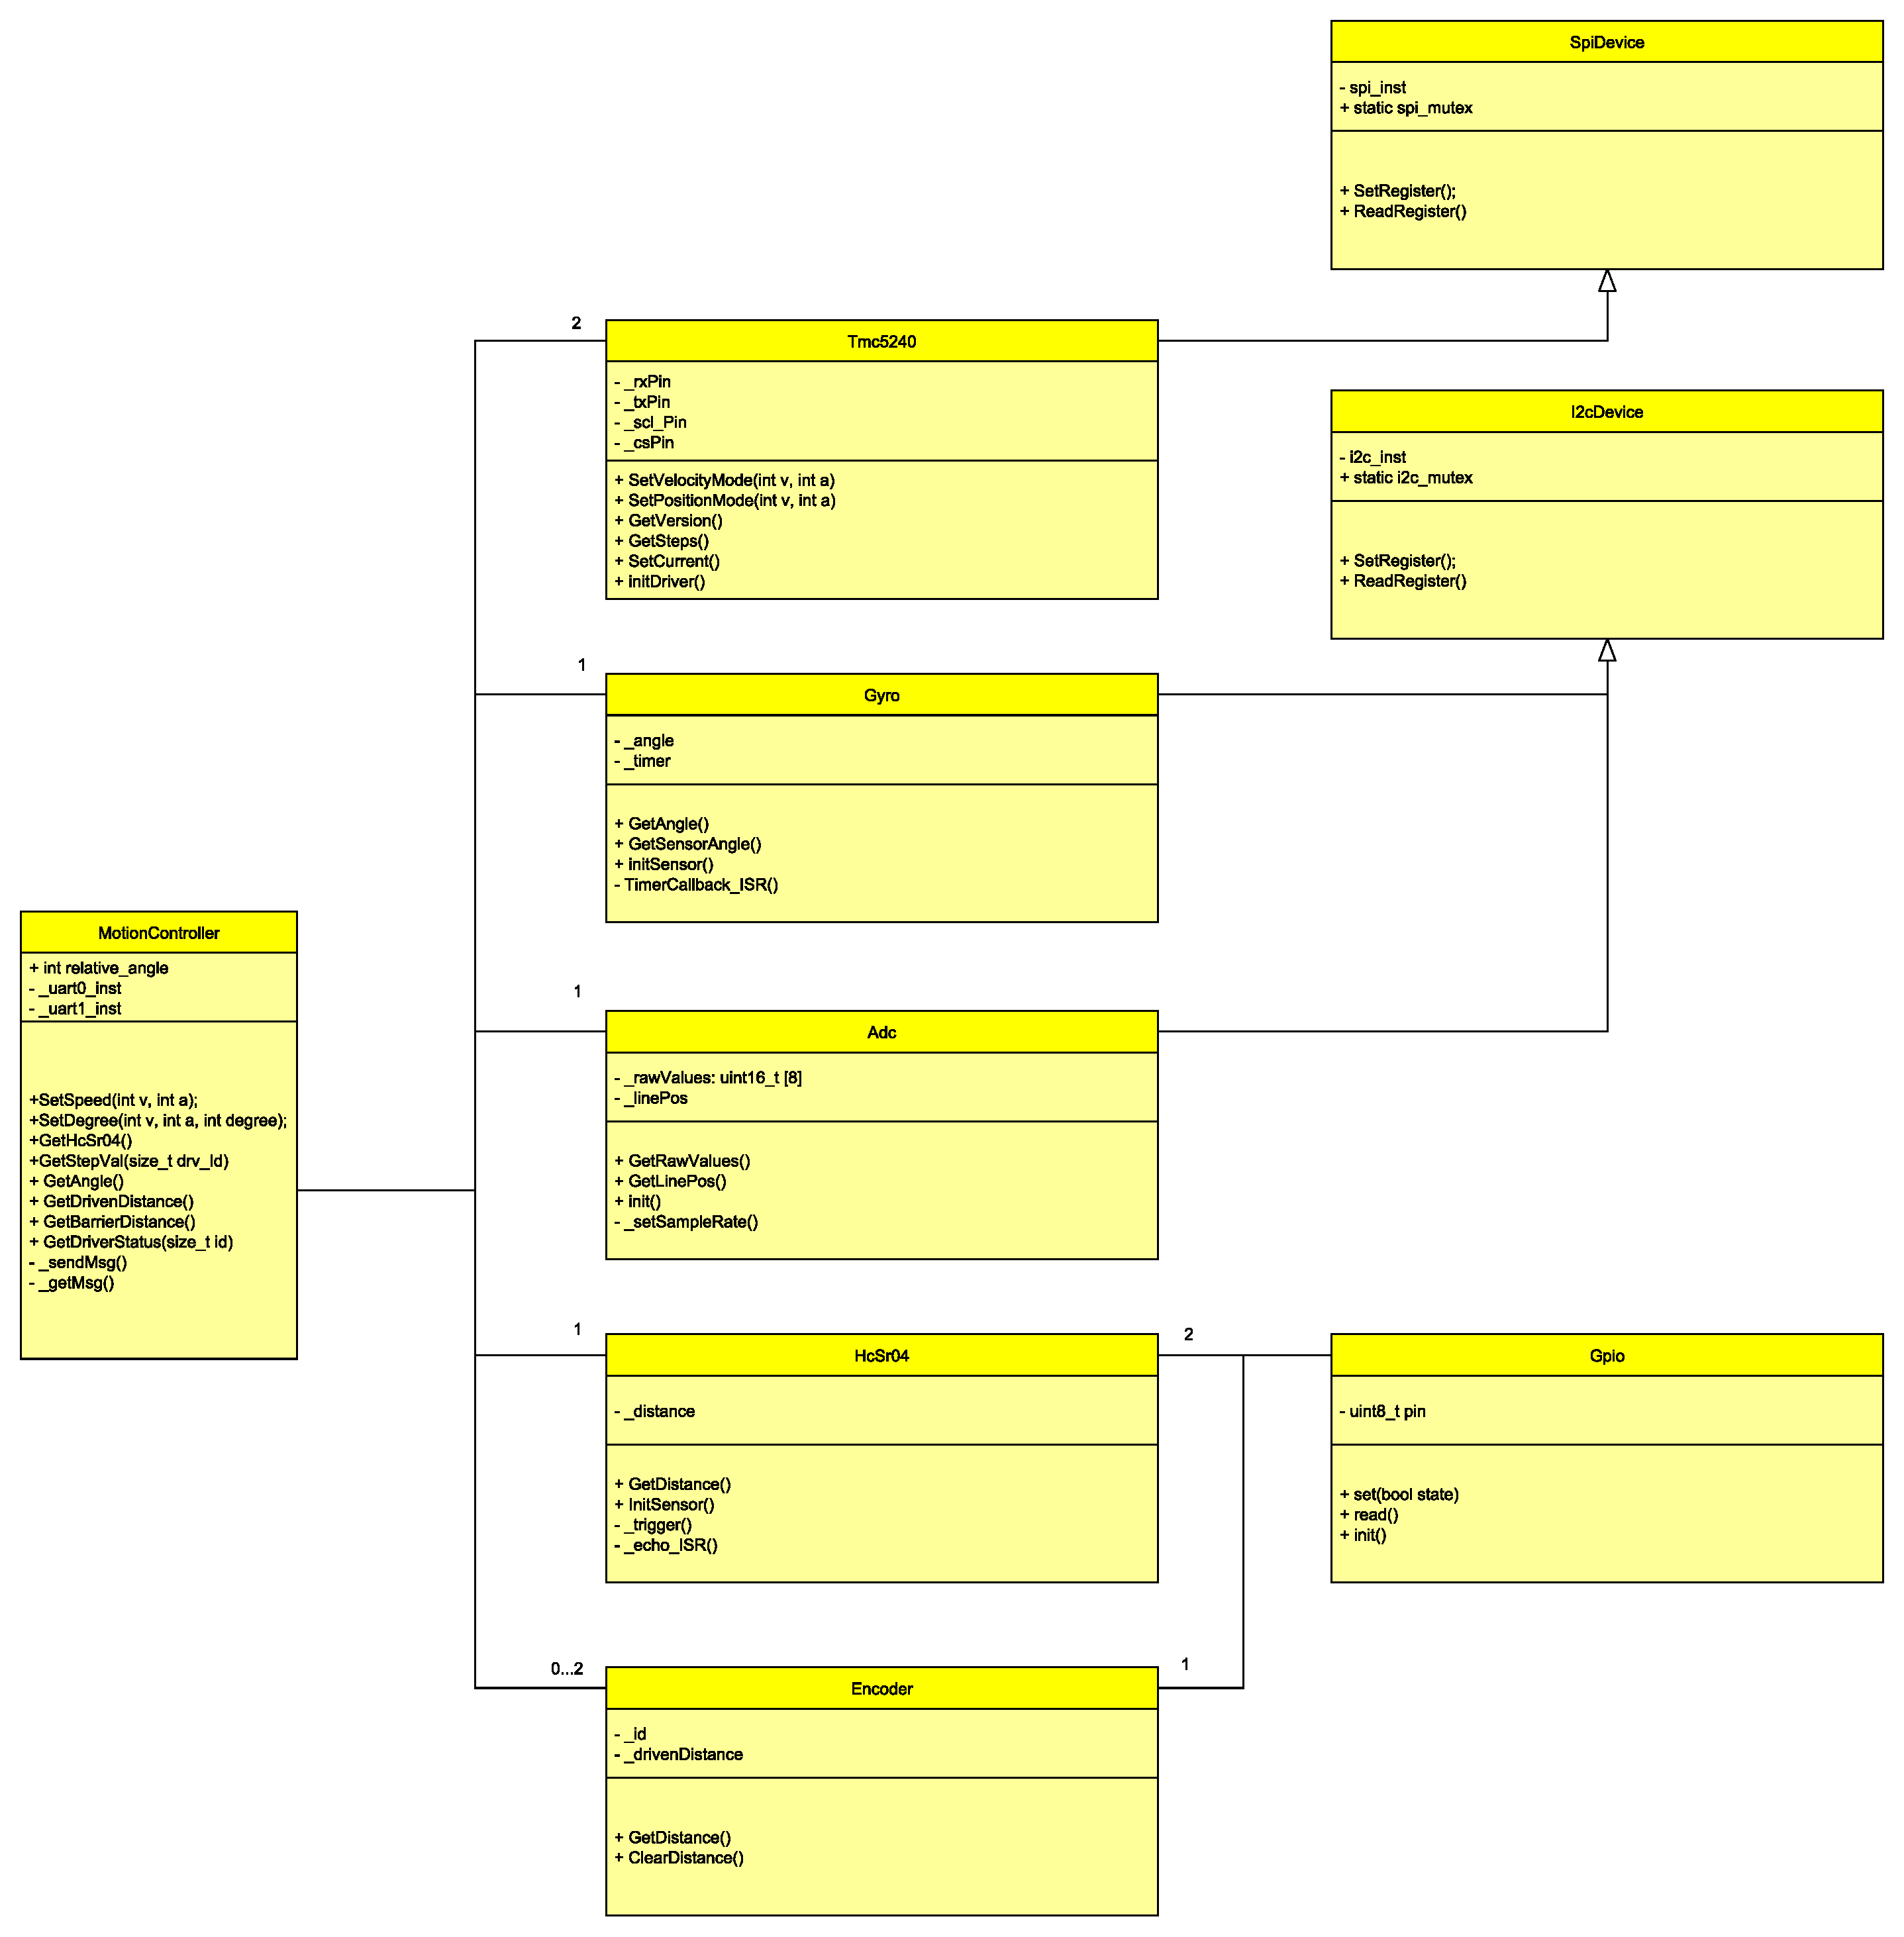
\includegraphics[width = 0.75\linewidth]{fig_Antriebe_und_Dimensionierung/Konzept_ClassDiagramm.pdf}
    \caption{Klassendiagramm Motion Controller}~\label{fig:MotionController_ClassDiagramm}
\end{figure}

In Abbildung~\ref{fig:MotionController_ClassDiagramm} ist konzeptionell
dargestellt, wie die zu erstellenden Klassen und Objekte in Beziehung
zueinander stehen werden.